\documentclass[11pt,twoside]{article}

\usepackage{amsmath}
\usepackage{amssymb}
\usepackage{amsthm}
\usepackage{courier} % Required for the courier font
\usepackage{extramarks} % Required for headers and footers
\usepackage{fancyhdr} % Required for custom headers
\usepackage{graphicx} % Required to insert images
\usepackage{lastpage} % Required to determine the last page for the footer
\usepackage{listings} % Required for insertion of code
\usepackage{lipsum} % Used for inserting dummy 'Lorem ipsum' text into the template
\usepackage{mathtools}
\usepackage{subcaption}

\usepackage[margin=1in]{geometry}
\usepackage[usenames,dvipsnames]{color} % Required for custom colors

\begin{document}

\title{CSC411 - Project \#3}
\author{Yui Chit (Michael) Wong - 999806232\\Yijin (Catherine) Wang - 998350476}
\maketitle

\clearpage

\section*{Part 1}
\paragraph{Question}
Describe the datasets. You will be predicting whether the review is positive or negative from keywords that appear in the review. Is that feasible? Give 3 examples of specific keywords that may be useful, together with statistics on how often they appear in positive and negative reviews.

\paragraph{Answer}
It is feasible. The word "best" appears in 489 positive reviews and 365 negative reviews. The word "horrendous" appears in 3 positive reviews and 9 negative reviews. The word "awful" appears in 19 positive reviews and 103 negative reviews. Therefore, "best" could be useful to identify positive review, while "horrendous" and "awful" could be used to identify negative review.  (There are 1000 positive reviews and 1000 negative reviews in total.)

\clearpage

\section*{Part 2}

\paragraph{Question}
Implement the Naive Bayes algorithm for predicting whether the review is positive or negative. Tune the parameter $m$ using the validation set, and report how you did it and what was the result. Report the performance on the training and the test sets that you obtain. Note that compting products of many small numbers leads to underflow. Use the fact that $a_1a_2\cdots a_n = exp(loga_1 + loga_2 + \cdots loga_n)$. In your report, explain how you used that fact.

\paragraph{Answer}
In order to predict the review, we use the formula:
\[P(class | a_1, \cdots, a_n) = \frac{P(a_1, \cdots, a_n | class) P(class)}{P(a_1, \cdots, a_n)}\]
If $P(positive|a_1, \cdots, a_n) \geq P(negative|a_1, \cdots, a_n)$, we predict the review to be positive. Otherwise, we predict the review to be negative. Because $P(a_1, \cdots, a_n)$ is the same for $P(positive|a_1, \cdots, a_n)$ and $P(negative|a_1, \cdots, a_n)$, we only need to compare $P(a_1, \cdots, a_n | positive) P(positive)$ and\\ $P(a_1, \cdots, a_n | negative) P(negative)$.
\begin{align*}
P(a_1, \cdots, a_n | class) P(class) &= P(a_1|class) P(a_2|class)\cdots P(a_n|class)P(class)\\
&= exp(log(P(a_1|class))+\cdots+log(P(a_n|class))+log(P(class)))
\end{align*}
Based on the formula above, we only need to compare $log(P(a_1|positive))+\cdots+log(P(a_n|positive))+log(P(positive))$ and $log(P(a_1|negative))+\cdots+log(P(a_n|negative))+log(P(negative))$. Therefore, we implemented our part 2 python program based on the comparison.
\clearpage

\section*{Part 3}

\paragraph{Question}
List the 10 words that most strongly predict that the review is positive, and the 10 words that most strongly predict that the review is negative. State how you obtained those in terms of the the conditional probabilities used in the Naive Bayes algorithm.

\paragraph{Answer}
\begin{align*}
P(class | a_i) &= \frac{P(a_i | class) P(class)}{P(a_i)}\\
P(class | a_i) &= exp(log(P(a_i | class)) + log(P(class)) - log(P(a_i)))
\end{align*}
We use the formula above to compute and compare $P(positive | a_i)$ for all words in positive reviews and $P(negative | a_i)$ for all words in negative reviews.\\
The top 10 words that predicts positive are:\\
'ziembicki', 'unites', 'ulu', 'torrance', 'toiling', 'tiegs', 'swope', 'salability', 'rothchild', 'rollergirl'\\
The top 10 words that predicts negative are:\\
'zaltar', 'workout', 'unmercifully', 'szwarc', 'stuffing', 'slunk', 'salkinds', 'refugees', 'popeye', 'omegahedron'\\
\clearpage

\section*{Part 4}
\paragraph{Question}
Train a Logistic Regression model on the same dataset. For a single movie review, For a single review $r$ the input to the Logistic Regression model will be a $k$-dimensional vector $v$ , where $v[k]=1$ if the $k$-th keyword appears in the review $r$. The set of keywords consists of all the words that appear in all the reviews.

Plot the learning curves (performance vs. iteration) of the Logistic Regression model. Describe how you selected the regularization parameter (and describe the experiments you used to select it).

\paragraph{Answer}
When working on this part of the project, we first obtained the whole list of keywords from the training set (both positive and negative reviews). Then for each review in the testing and validation set, we will create a $k$-dimensional vector $v$, where $v[k]=1$ if the $k$-th keyword appears in the review. If a review from the test or validation set contains a keyword that isn't in the training keyword set, it would be ignored. We then stack the vectors together to get a `$x$' for each of the training, test, and validation. 

We then used the $x\_train$ to train the model and test the performance on $x\_test, x\_val$. We used tensorflow to implement the architecture of the model. We used one-hot encoding for the output. For the network model, we only have 1 input layer and an output layer that has sigmoid activiation function. We also have a $L2$ penalty for the weight (used as regularization). The training step is done by the Adam Optimizer, which is a variant of gradient descend. Also, each iteration we will take a randomly chosen mini batch from the original training set to speed the process and avoid running into local minima.

When picking the parameter, it's done mostly by trial and error. We tested different values for the parameters, and selected the best one based on the performance on validation.

I ran the training step for 10000 iterations, and the final performance on training set and test set are 100\% and 86\% respectively. The result of the training vs. iteration is summarized below:

\begin{figure*}[h]
	\centering
	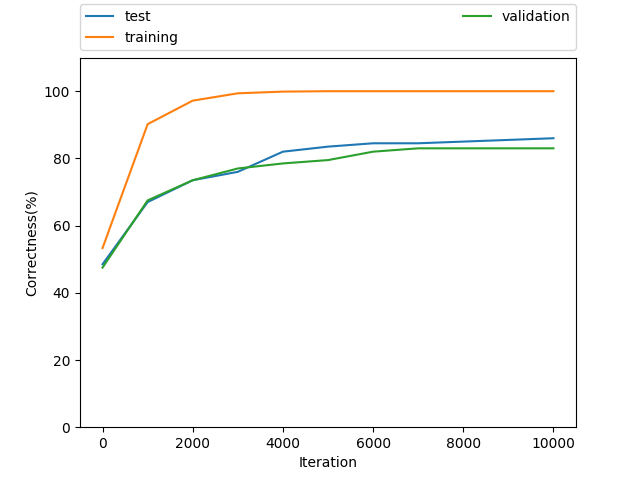
\includegraphics[scale=0.8]{part4.png}
	\caption*{Learning curve}
\end{figure*}

\clearpage

\section*{Part 5}
\paragraph{Question}
At test time, both Logistic Regression and Naive Bayes can be formulated as computing

\[\theta_0+\theta_1I_1(x)+\theta_2I_2(x)+\cdots+\theta_kI_k(x) > thr\]

in order to decide whether to classify $x$ as 1 or 0 . Explain, in each case, what the $\theta$‘s and the $I$‘s are.

\paragraph{Answer}
Assume $x$ is one review which is a $k$-dimensional vector where $k$ is the total number of unique words in the set.\\
$\theta_0$ is the bias.\\
$I_i(x)$ is the $i$th word of input $x$. $I_i(x)$ is either 1 or 0, where 1 means that $i$th word is in review $x$, 0 means that $i$th word is not in review $x$.\\
$\theta_i$ is $log(P(word_i | positive))  - log(P(word_i | negative))$
\clearpage

\section*{Part 6}
\paragraph{Question}

\paragraph{Answer}


\clearpage

\section*{Part 7}
\paragraph{Question}


\paragraph{Answer}


\clearpage

\section*{Part 8}
\paragraph{Question}


\paragraph{Answer}


\clearpage


\end{document}